\documentclass[11pt,a4paper]{article}

\usepackage[utf8]{inputenc}
\usepackage[T1]{fontenc}
\usepackage{lmodern}
\usepackage[margin=2.5cm]{geometry}
\usepackage{microtype}
\usepackage{amsmath,amssymb}
\usepackage{graphicx}
\usepackage{subcaption}
\usepackage{booktabs}
\usepackage{array}
\usepackage{xcolor}
\usepackage{enumitem}
\usepackage{float}
\usepackage{listings}
\usepackage{tikz}
\usetikzlibrary{arrows.meta,positioning,calc,fit,backgrounds}
\usepackage[hidelinks]{hyperref}

\graphicspath{{figures/}}
\setlength{\parindent}{0pt}
\setlength{\parskip}{0.6em}
\setlist{itemsep=0.2em,topsep=0.3em}

% ---------- colours and TikZ styles ----------
\definecolor{inc}{HTML}{1F9D63}
\definecolor{outc}{HTML}{D1433B}
\definecolor{undecc}{HTML}{B7790C}
\definecolor{accent}{HTML}{2457D6}

\tikzset{
  arg/.style={circle,draw=#1,fill=#1!12,line width=1pt,minimum size=8mm,inner sep=0pt,font=\small\bfseries},
  arg/.default=undecc,
  atk/.style={-{Stealth[length=2.4mm]},thick,gray!70!black},
  owner/.style={font=\scriptsize\itshape,text=gray!60!black},
  box/.style={draw=accent,fill=accent!6,rounded corners=2pt,align=center,inner sep=5pt,font=\small},
  flow/.style={-{Stealth[length=2.4mm]},thick,accent}
}

\lstset{
  basicstyle=\ttfamily\footnotesize,
  frame=single,
  rulecolor=\color{gray!50},
  breaklines=true,
  columns=fullflexible,
  keepspaces=true
}

\newcommand{\AF}{\mathit{AF}}
\newcommand{\attacks}{\rightharpoonup}
\newcommand{\file}[1]{\texttt{#1}}

\title{Argument Lab: Exact Abstract Argumentation and\\Strategic Argument Revelation}
\author{Jatin Purbia (B23CH1022) \and Sharana Gouda Lakshetty (B23CH1042)\\[0.5em]\normalsize Autonomous Systems --- Assignment 03}
\date{\today}

\begin{document}
\maketitle

\begin{abstract}
\noindent
This report describes \emph{Argument Lab}, a local application for abstract argumentation and for the strategic question of whether an agent can profit from hiding arguments. The system implements Dung's abstract argumentation frameworks with exact enumeration of the grounded, complete, preferred, stable and semi-stable semantics, legal labellings and acceptance status. On top of that it implements the grounded direct mechanism of Chapter~5 of \emph{Multiagent Systems} (Weiss, 2013): best responses, an exhaustive check of strategyproofness (Theorem~5.3) and a separate check of the structural sufficient condition (Theorem~5.4). We validate the implementation against the textbook examples and against independent oracles over all 512 directed three-node graphs, and we run a seeded experiment of 5{,}000 random three-agent instances. Of these, 1{,}054 are strategyproof; the fraction falls from 83.7\% at attack probability $p=0.1$ to 0.1\% at $p=0.9$. The structural condition held in 285 instances and \emph{every} one of them was strategyproof, while 769 further instances were strategyproof although the condition failed. An independent audit confirmed all 5{,}000 decisions.
\end{abstract}

\tableofcontents
\newpage

% =====================================================================
\section{Introduction}
Argumentation is a way of reasoning in which conclusions are justified by arguments that can attack one another. In \emph{abstract} argumentation the content of an argument is ignored: only the attack relation between arguments matters. This is enough to define precisely which sets of arguments can be accepted together, and different definitions of ``acceptable'' give different \emph{semantics}.

When the arguments are put forward by self-interested agents, a second question appears. An agent decides which of its arguments to reveal, and revealing more arguments can change the outcome in ways that hurt the agent itself. A mechanism is \emph{strategyproof} when revealing everything is always at least as good as any other report, whatever the other agents do.

The goals of this project are:
\begin{enumerate}
  \item implement abstract argumentation frameworks and the five standard semantics exactly;
  \item implement the grounded direct mechanism, its best responses, and checks of Theorems~5.3 and~5.4;
  \item reproduce the textbook examples, including two textbook errata;
  \item run a reproducible random experiment and relate the structural condition to measured strategyproofness;
  \item make all of this explorable in a local browser application.
\end{enumerate}

The reference is Chapter~5 of G.~Weiss (ed.), \emph{Multiagent Systems}, 2nd ed., MIT Press, 2013 (printed pp.~181--185 and 199--201). ASCII names $a_1,a_2,\dots$ stand for the book's indexed arguments.

% =====================================================================
\section{Background}
\subsection{Abstract argumentation frameworks}
An argumentation framework is a pair $\AF=(A,R)$ where $A$ is a finite set of arguments and $R\subseteq A\times A$ is the attack relation; $(a,b)\in R$ is written $a\attacks b$. Self-attacks, mutual attacks and arbitrary directed cycles are all permitted. For $S\subseteq A$ let $S^{+}=\{b\mid \exists a\in S:\ a\attacks b\}$ be the set of arguments attacked by $S$.

\begin{itemize}
  \item $S$ is \emph{conflict-free} iff $S\cap S^{+}=\emptyset$.
  \item $S$ \emph{defends} $a$ iff every attacker of $a$ lies in $S^{+}$. An unattacked argument is defended by every set, including $\emptyset$.
  \item The \emph{characteristic function} is $F(S)=\{a\in A\mid S\text{ defends }a\}$. It is monotone, and $F(S)$ may contain arguments outside $S$.
\end{itemize}

Table~\ref{tab:semantics} lists the semantics implemented. Preferred and semi-stable use \emph{set inclusion} for maximality, never cardinality: an incomparable extension is not discarded because another one is larger.

\begin{table}[H]
\centering
\caption{Semantics implemented in the engine.}
\label{tab:semantics}
\small
\begin{tabular}{@{}p{3cm}p{11.5cm}@{}}
\toprule
Semantics & Definition \\
\midrule
Admissible & $S$ is conflict-free and $S\subseteq F(S)$. \\
Complete & $S$ is conflict-free and $S=F(S)$. \\
Grounded & The least fixed point of $F$, obtained by iterating $F$ from $\emptyset$ until nothing changes. It exists and is unique. \\
Preferred & An inclusion-maximal complete (equivalently, admissible) set. \\
Stable & $S$ is conflict-free and $S^{+}=A\setminus S$. May not exist (for example on an odd cycle). \\
Semi-stable & A complete set whose \emph{range} $S\cup S^{+}$ is inclusion-maximal. \\
\bottomrule
\end{tabular}
\end{table}

\subsection{Labellings and acceptance status}
A \emph{labelling} assigns each argument one of \textsf{in}, \textsf{out} or \textsf{undec}. It is \emph{legal} when an argument is \textsf{in} iff all its attackers are \textsf{out}, and \textsf{out} iff at least one attacker is \textsf{in}. Every complete extension $S$ yields exactly one legal labelling: $\textsf{in}=S$, $\textsf{out}=S^{+}$ and $\textsf{undec}=A\setminus(S\cup S^{+})$. The implementation uses this bijection rather than testing all $3^{|A|}$ candidate labellings.

Given a semantics, an argument is \emph{skeptically accepted} if it is in every extension, \emph{credulously accepted} if it is in some but not all, and \emph{rejected} if it is in none. If a semantics has no extension (stable semantics on an odd cycle), acceptance is reported as \emph{undefined} rather than vacuously accepting every argument.

\subsection{Strategic revelation}
Let the arguments be partitioned into ownership sets $A_1,\dots,A_m$, one per agent. Agent $i$ may reveal any subset $R_i\subseteq A_i$, including $\emptyset$, but cannot reveal another agent's arguments. The \emph{grounded direct mechanism} takes the revealed arguments $\bigcup_i R_i$, induces the framework on them, and outputs its grounded extension $G(R_1,\dots,R_m)$. The utility of agent $i$ is
\[
u_i(R_1,\dots,R_m)=\bigl|\,G(R_1,\dots,R_m)\cap A_i\,\bigr|,
\]
the number of \emph{its own} arguments that are accepted, not the global number of accepted arguments.

Truthful revelation is a \emph{dominant strategy} for agent $i$ iff for every report profile $R_{-i}$ of the others and every $R_i\subseteq A_i$ we have $u_i(A_i,R_{-i})\ge u_i(R_i,R_{-i})$. The mechanism is \emph{strategyproof} if this holds for every agent (Theorem~5.3 of the book). Theorem~5.4 gives a structural \emph{sufficient} condition: no agent owns two arguments connected by a directed odd-length path in the full framework. The failure of that condition does not by itself imply manipulability.

% =====================================================================
\section{Algorithms}
\subsection{Exact enumeration of semantics}
For frameworks of at most 12 arguments, the engine enumerates all $2^{|A|}$ subsets once, keeps the conflict-free ones, and derives the semantics from them. Complete extensions are the conflict-free fixed points of $F$; preferred, stable and semi-stable extensions are filtered from them by inclusion-maximality, range-maximality and the stable condition. The grounded extension is computed by direct iteration, which also yields the \emph{trace} $\emptyset\to F(\emptyset)\to F^{2}(\emptyset)\to\dots$ shown in the interface.

\subsection{Best responses and the strategyproofness check}
For an agent $i$ and fixed reports $R_{-i}$ of the others, \emph{best-response enumeration} evaluates all $2^{|A_i|}$ own reports and returns \emph{every} report that attains the maximum utility. Ties matter because truthful reporting need only be a weak best response.

The Theorem~5.3 check enumerates every agent, every combination of the \emph{other} agents' reports (they are not restricted to be truthful) and every own report, and compares each with full revelation. A strictly better alternative disproves strategyproofness and is returned as a \emph{witness}: the agent, the others' reports, the truthful and deviating reports, both outcomes and both utilities. If none exists, truthful reporting is weakly dominant for all agents. Writing $n=|A|$ and $m$ for the number of agents, the complete check compares $m\cdot 2^{n}$ reports against the truthful one. Figure~\ref{fig:cost} confirms that every strategyproof instance in the experiment used exactly $3\cdot2^{n}$ comparisons.

\begin{figure}[H]
\centering
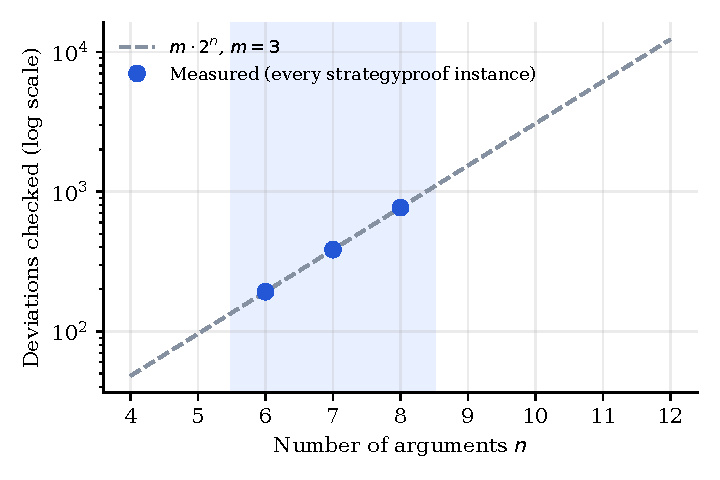
\includegraphics[width=0.62\textwidth]{fig_comparisons_by_n.pdf}
\caption{Number of deviations compared by the exhaustive check for strategyproof instances ($m=3$ agents). Measured values coincide with $m\cdot2^{n}$ for $n=6,7,8$; the dashed curve extrapolates to the interface's limit of $n=12$.}
\label{fig:cost}
\end{figure}

\subsection{The odd-walk condition}
The structural condition is evaluated separately and never used as a shortcut for the exhaustive check. It asks whether some agent owns arguments $a,b$ such that an odd-length directed path leads from $a$ to $b$. The implementation adopts the documented \emph{directed-walk} convention: vertices may repeat, and same-endpoint odd cycles count. From each source a breadth-first search explores states $(\text{vertex},\text{parity})$, flipping the parity on each attack. There are at most $2|A|$ states per source, so cycles terminate, and the total cost is $O\bigl(n(n+|R|)\bigr)$. This convention is conservative: under a stricter simple-path reading the condition can hold in more graphs. A failed condition is therefore reported only as a failure of a \emph{sufficient} condition.

% =====================================================================
\section{System design}
\subsection{Architecture}
Figure~\ref{fig:architecture} shows the structure. The domain layer is pure Python and independent of HTTP. A thin adapter layer validates requests, runs use cases and manages background jobs. The browser frontend is plain HTML, CSS and JavaScript served by the same process; it contains no algorithms.

\begin{figure}[H]
\centering
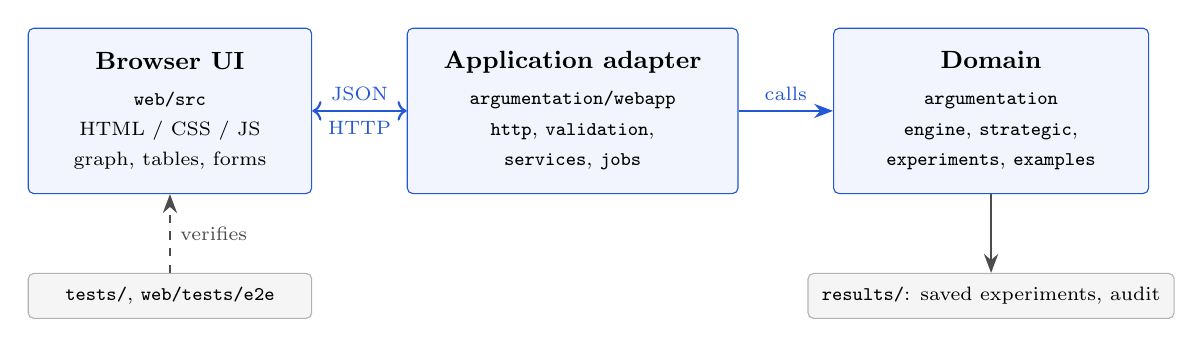
\begin{tikzpicture}[node distance=9mm and 12mm]
  \node[box,minimum width=3.6cm,minimum height=2.1cm] (ui) {\textbf{Browser UI}\\[2pt]\scriptsize \file{web/src}\\\scriptsize HTML / CSS / JS\\\scriptsize graph, tables, forms};
  \node[box,minimum width=4.2cm,minimum height=2.1cm,right=of ui] (app) {\textbf{Application adapter}\\[2pt]\scriptsize \file{argumentation/webapp}\\\scriptsize \texttt{http}, \texttt{validation},\\\scriptsize \texttt{services}, \texttt{jobs}};
  \node[box,minimum width=4.0cm,minimum height=2.1cm,right=of app] (dom) {\textbf{Domain}\\[2pt]\scriptsize \file{argumentation}\\\scriptsize \texttt{engine}, \texttt{strategic},\\\scriptsize \texttt{experiments}, \texttt{examples}};
  \draw[flow,<->] (ui) -- node[above,font=\scriptsize]{JSON} node[below,font=\scriptsize]{HTTP} (app);
  \draw[flow] (app) -- node[above,font=\scriptsize]{calls} (dom);
  \node[box,fill=gray!8,draw=gray!60,below=10mm of dom,minimum width=4.0cm] (res) {\scriptsize \file{results/}: saved experiments, audit};
  \node[box,fill=gray!8,draw=gray!60,below=10mm of ui,minimum width=3.6cm] (tests) {\scriptsize \file{tests/}, \file{web/tests/e2e}};
  \draw[flow,gray!60!black] (dom) -- (res);
  \draw[flow,gray!60!black,dashed] (tests) -- node[right,font=\scriptsize]{verifies} (ui);
\end{tikzpicture}
\caption{Layered architecture. Dependencies point left to right; the domain does not know about HTTP or the UI.}
\label{fig:architecture}
\end{figure}

Table~\ref{tab:modules} summarises the responsibilities of each module.

\begin{table}[H]
\centering
\caption{Source modules and their responsibilities.}
\label{tab:modules}
\small
\begin{tabular}{@{}p{4.3cm}p{10.2cm}@{}}
\toprule
Module & Responsibility \\
\midrule
\file{engine.py} & \texttt{ArgumentationFramework}: conflict-freeness, defence, $F$, admissible/complete/grounded/preferred/stable/semi-stable extensions, legal labellings, acceptance. \\
\file{strategic.py} & \texttt{GroundedMechanism}: ownership, reports, induced outcome, utilities, best responses, Theorem~5.3 check, Theorem~5.4 condition. \\
\file{experiments.py} & Seeded instance generation and the batch runner that writes the saved results. \\
\file{examples.py} & Named fixtures (textbook figures and examples) shown in the interface. \\
\file{webapp/validation.py} & Parses request JSON into domain objects and rejects malformed input. \\
\file{webapp/services.py} & Use cases: \texttt{analyse} and \texttt{strategic}. \\
\file{webapp/jobs.py} & Background experiment jobs: one active job, five retained, polled by the browser. \\
\file{webapp/http.py} & HTTP routing, payload and content-type limits, same-origin check on writes, static files; binds to \texttt{127.0.0.1}. \\
\bottomrule
\end{tabular}
\end{table}

\subsection{HTTP interface}
\begin{table}[H]
\centering
\caption{Routes served by the local application.}
\small
\begin{tabular}{@{}p{4.8cm}p{9.7cm}@{}}
\toprule
Route & Purpose \\
\midrule
\texttt{GET /api/health} & Readiness and version. \\
\texttt{GET /api/examples} & Fixture frameworks with ownership. \\
\texttt{POST /api/analyse} & Extensions, labellings, set checks and acceptance for a framework. \\
\texttt{POST /api/strategic} & Outcome, utilities, strategyproofness, best responses. \\
\texttt{POST /api/experiments} & Start a background experiment; returns a job id. \\
\texttt{GET /api/jobs/<id>} & Poll job progress and result. \\
\texttt{GET /api/saved-experiments} & The submitted 5{,}000-instance results. \\
\bottomrule
\end{tabular}
\end{table}

The application has no third-party Python dependency, no external API and needs no internet connection. It is intended for a trusted local workstation: payload size, graph size and experiment size are bounded, and write routes reject cross-origin browser requests.

\subsection{User interface}
The interface has three workspaces, each fitting on one screen on a desktop display; on narrow screens the sections stack. The \emph{Framework studio} combines an editor, an interactive attack graph coloured by the grounded labelling, a quick check of an arbitrary set $S$, and tabs for extensions, acceptance status and labellings. The \emph{Strategic playground} shows each agent's arguments as toggles for hiding or revealing, and presents the utilities, both theorem verdicts and the full best-response table. The \emph{Experiments} workspace runs or loads experiments and shows summaries and individual instances.

% =====================================================================
\section{Validation on the textbook examples}
Every example below is a fixture in the application and an assertion in the test suite. In the figures, green nodes are \textsf{in} (grounded), red nodes are \textsf{out} and amber nodes are \textsf{undec}.

\begin{figure}[H]
\centering
\begin{subfigure}[t]{0.48\textwidth}
\centering
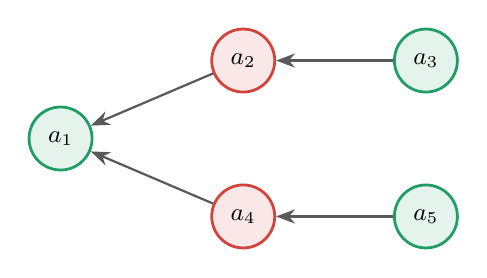
\begin{tikzpicture}[x=1.45cm,y=1.1cm]
  \node[arg=inc] (a1) at (0,0) {$a_1$};
  \node[arg=outc] (a2) at (1.6,0.9) {$a_2$};
  \node[arg=outc] (a4) at (1.6,-0.9) {$a_4$};
  \node[arg=inc] (a3) at (3.2,0.9) {$a_3$};
  \node[arg=inc] (a5) at (3.2,-0.9) {$a_5$};
  \draw[atk] (a2) -- (a1);
  \draw[atk] (a4) -- (a1);
  \draw[atk] (a3) -- (a2);
  \draw[atk] (a5) -- (a4);
\end{tikzpicture}
\caption{Figure 5.1: grounded $=\{a_1,a_3,a_5\}$.}
\end{subfigure}\hfill
\begin{subfigure}[t]{0.48\textwidth}
\centering
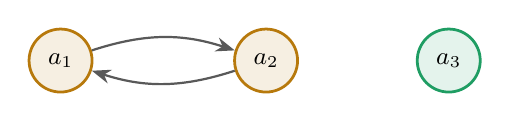
\begin{tikzpicture}[x=1.45cm,y=1.1cm]
  \node[arg=undecc] (b1) at (0,0.4) {$a_1$};
  \node[arg=undecc] (b2) at (1.8,0.4) {$a_2$};
  \node[arg=inc] (b3) at (3.4,0.4) {$a_3$};
  \draw[atk,bend left=18] (b1) to (b2);
  \draw[atk,bend left=18] (b2) to (b1);
\end{tikzpicture}
\caption{Figure 5.2: grounded $=\{a_3\}$.}
\end{subfigure}
\caption{Abstract frameworks from the textbook (Examples 5.5--5.8).}
\label{fig:book-abstract}
\end{figure}

\paragraph{Figure 5.1 (Examples 5.5, 5.6, 5.8).}
The attacks are $a_2\attacks a_1$, $a_4\attacks a_1$, $a_3\attacks a_2$, $a_5\attacks a_4$. The set $\{a_3,a_5\}$ is conflict-free and admissible, and it defends $a_1$, so it is not complete. Grounded iteration gives $\emptyset\to\{a_3,a_5\}\to\{a_1,a_3,a_5\}$, and this final set is the unique complete, preferred, stable and semi-stable extension.

\paragraph{Figure 5.2 (Examples 5.7, 5.8).}
$a_1$ and $a_2$ attack each other and $a_3$ is unattacked. The complete extensions are $\{a_3\}$, $\{a_1,a_3\}$ and $\{a_2,a_3\}$; the grounded extension is $\{a_3\}$; the preferred and stable extensions are $\{a_1,a_3\}$ and $\{a_2,a_3\}$. There are three legal labellings. Under preferred semantics $a_3$ is skeptically accepted and $a_1,a_2$ are credulously accepted.

\begin{figure}[H]
\centering
\begin{subfigure}[t]{0.48\textwidth}
\centering
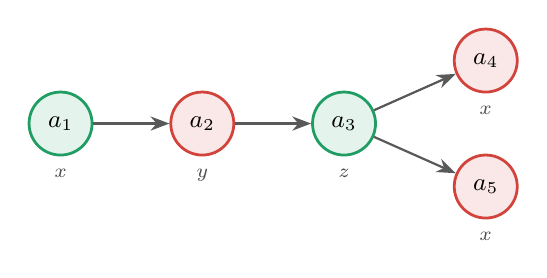
\begin{tikzpicture}[x=1.2cm,y=1cm]
  \node[arg=inc] (a1) at (0,0) {$a_1$};
  \node[arg=outc] (a2) at (1.5,0) {$a_2$};
  \node[arg=inc] (a3) at (3,0) {$a_3$};
  \node[arg=outc] (a4) at (4.5,0.8) {$a_4$};
  \node[arg=outc] (a5) at (4.5,-0.8) {$a_5$};
  \draw[atk] (a1) -- (a2);
  \draw[atk] (a2) -- (a3);
  \draw[atk] (a3) -- (a4);
  \draw[atk] (a3) -- (a5);
  \node[owner,below=1pt of a1] {$x$};
  \node[owner,below=1pt of a2] {$y$};
  \node[owner,below=1pt of a3] {$z$};
  \node[owner,below=1pt of a4] {$x$};
  \node[owner,below=1pt of a5] {$x$};
\end{tikzpicture}
\caption{Example 5.10 (full reports).}
\end{subfigure}\hfill
\begin{subfigure}[t]{0.48\textwidth}
\centering
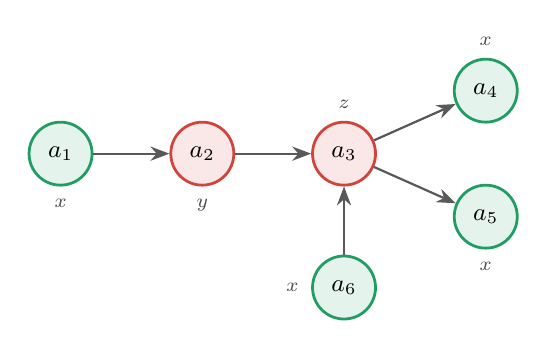
\begin{tikzpicture}[x=1.2cm,y=1cm]
  \node[arg=inc] (a1) at (0,0) {$a_1$};
  \node[arg=outc] (a2) at (1.5,0) {$a_2$};
  \node[arg=outc] (a3) at (3,0) {$a_3$};
  \node[arg=inc] (a4) at (4.5,0.8) {$a_4$};
  \node[arg=inc] (a5) at (4.5,-0.8) {$a_5$};
  \node[arg=inc] (a6) at (3,-1.7) {$a_6$};
  \draw[atk] (a1) -- (a2);
  \draw[atk] (a2) -- (a3);
  \draw[atk] (a3) -- (a4);
  \draw[atk] (a3) -- (a5);
  \draw[atk] (a6) -- (a3);
  \node[owner,below=1pt of a1] {$x$};
  \node[owner,below=1pt of a2] {$y$};
  \node[owner,above=1pt of a3] {$z$};
  \node[owner,above=1pt of a4] {$x$};
  \node[owner,below=1pt of a5] {$x$};
  \node[owner,left=1pt of a6] {$x$};
\end{tikzpicture}
\caption{Example 5.11 (full reports).}
\end{subfigure}
\caption{The strategic examples. Letters below nodes give the owning agent; colouring shows the grounded outcome of the fully revealed framework.}
\label{fig:book-strategic}
\end{figure}

\paragraph{Example 5.10.}
Agent $x$ owns $\{a_1,a_4,a_5\}$, $y$ owns $\{a_2\}$ and $z$ owns $\{a_3\}$. With full reports the grounded outcome is $\{a_1,a_3\}$ and the utilities are $(1,0,1)$. If $x$ hides $a_1$, the outcome becomes $\{a_2,a_4,a_5\}$ and $x$'s utility rises to 2: a strictly profitable deviation. \emph{Erratum:} the book's utility sentence swaps $y$ and $z$; the implementation and tests use the values above.

\paragraph{Example 5.11.}
Adding $a_6$, owned by $x$, with $a_6\attacks a_3$ gives the full-report outcome $\{a_1,a_4,a_5,a_6\}$ and utility 4 for $x$. The exhaustive check verifies truthfulness against \emph{every} profile of the others, not just this one. The odd-walk condition nevertheless \emph{fails} because of $a_1\attacks a_2\attacks a_3\attacks a_4$. So this is a strategyproof framework in which the sufficient condition does not hold. \emph{Erratum:} the argument that neutralises the indirect self-defeat is $a_6$, not $a_5$ as written in the discussion in the book.

\paragraph{Further fixtures.}
The tests also cover a defence chain, mutual attack, an odd cycle (no stable extension, all arguments undecided; Figure~\ref{fig:oddcycle}), self-attacks, the empty framework, agents with no arguments, and harmless internal conflict.

\begin{figure}[H]
\centering
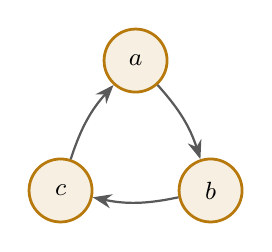
\begin{tikzpicture}
  \node[arg=undecc] (c1) at (90:1.1) {$a$};
  \node[arg=undecc] (c2) at (-30:1.1) {$b$};
  \node[arg=undecc] (c3) at (210:1.1) {$c$};
  \draw[atk] (c1) to[bend left=12] (c2);
  \draw[atk] (c2) to[bend left=12] (c3);
  \draw[atk] (c3) to[bend left=12] (c1);
\end{tikzpicture}
\caption{Odd cycle $a\attacks b\attacks c\attacks a$: the only complete extension is $\emptyset$, there is no stable extension, and stable acceptance is reported as undefined.}
\label{fig:oddcycle}
\end{figure}

% =====================================================================
\section{Experimental method}
The submitted experiment samples 1{,}000 instances for each of five attack probabilities $p\in\{0.1,0.3,0.5,0.7,0.9\}$, in total 5{,}000 instances, with Python's seeded generator (seed 2026). The assignment text omitted the probability values; these are explicit provisional choices and are stored with the results.
\begin{itemize}
  \item The number of arguments $n$ is uniform on $\{6,7,8\}$.
  \item Each ordered pair of distinct arguments is an attack independently with probability $p$. Directed cycles are allowed; self-attacks are excluded by default (a command-line and browser option enables them).
  \item Each argument is assigned independently and uniformly to one of three agents, rejecting assignments in which some agent is empty. Ownership is thus uniform over surjective assignments, not over size vectors.
  \item The random stream continues across probability groups in the stated order.
\end{itemize}
Every instance runs the exhaustive Theorem~5.3 check and, separately, the Theorem~5.4 condition. Each record keeps the graph, ownership, both flags, the number of comparisons and any witness, so every exceptional instance is identifiable.

To check the generator, Figure~\ref{fig:generator} compares the measured mean number of attacks with the expectation $p\,\mathbb{E}[n(n-1)]=p\cdot 42.67$; they agree closely.

\begin{figure}[H]
\centering
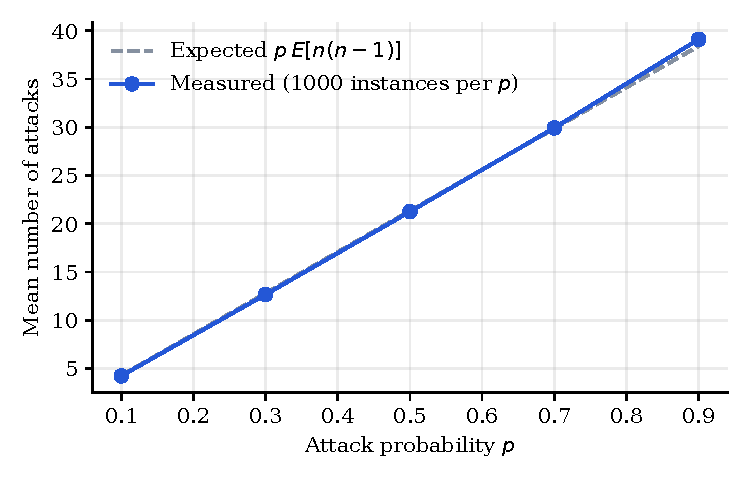
\includegraphics[width=0.6\textwidth]{fig_generator_check.pdf}
\caption{Sanity check of the random-graph generator.}
\label{fig:generator}
\end{figure}

% =====================================================================
\section{Results}
\subsection{Strategyproofness against attack density}
Table~\ref{tab:results} and Figure~\ref{fig:sp-fraction} show that strategyproofness becomes rare as the attack graph gets denser: 83.7\% of instances at $p=0.1$, falling to 0.1\% at $p=0.9$. Overall 1{,}054 of 5{,}000 instances (21.1\%) were strategyproof. Intervals in the table are 95\% Wilson score intervals for a binomial proportion of 1{,}000 trials. This is an empirical statement about the specified generator and seed; it is not a proof of monotonicity.

\begin{table}[H]
\centering
\caption{Results by attack probability (1{,}000 instances each). ``SP'' means strategyproof.}
\label{tab:results}
\footnotesize
\begin{tabular}{@{}rrrrrrr@{}}
\toprule
$p$ & SP & Fraction & 95\% interval & Cond.\ holds & Holds, not SP & SP, cond.\ fails \\
\midrule
0.1 & 837 & 0.837 & [0.813, 0.859] & 276 & 0 & 561 \\
0.3 & 188 & 0.188 & [0.165, 0.213] & 9 & 0 & 179 \\
0.5 & 24 & 0.024 & [0.016, 0.035] & 0 & 0 & 24 \\
0.7 & 4 & 0.004 & [0.002, 0.010] & 0 & 0 & 4 \\
0.9 & 1 & 0.001 & [0.000, 0.006] & 0 & 0 & 1 \\
\midrule
Total & 1054 & 0.211 & & 285 & 0 & 769 \\
\bottomrule
\end{tabular}
\end{table}

\begin{figure}[H]
\centering
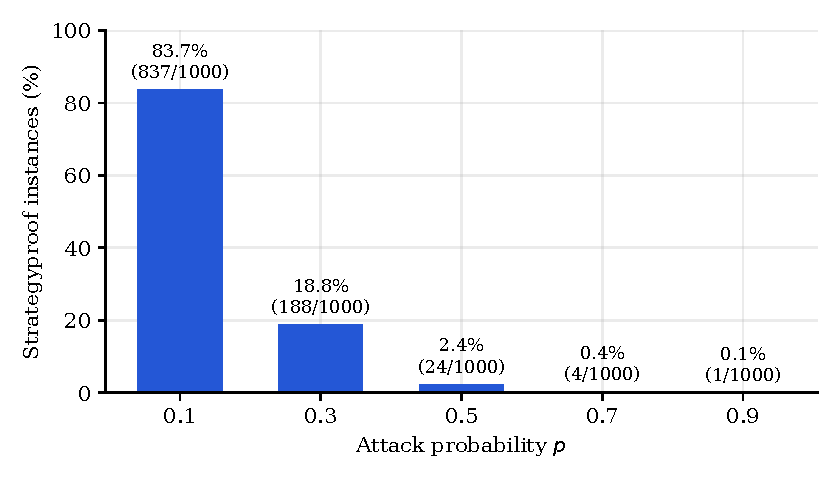
\includegraphics[width=0.7\textwidth]{fig_strategyproof_fraction.pdf}
\caption{Fraction of strategyproof instances by attack probability.}
\label{fig:sp-fraction}
\end{figure}

Splitting by instance size (Figure~\ref{fig:heatmap}) shows that larger graphs are less often strategyproof at every density: at $p=0.1$ the fraction falls from 90.7\% for $n=6$ to 74.3\% for $n=8$, and at $p=0.3$ from 32.9\% to 7.7\%. More arguments mean more opportunities to hide something profitably.

\begin{figure}[H]
\centering
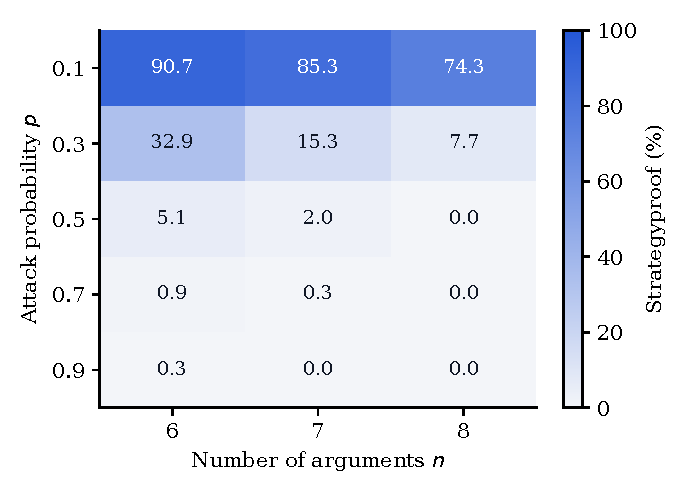
\includegraphics[width=0.62\textwidth]{fig_heatmap_p_n.pdf}
\caption{Percentage of strategyproof instances by attack probability and number of arguments.}
\label{fig:heatmap}
\end{figure}

\subsection{The structural condition versus measured strategyproofness}
Figure~\ref{fig:breakdown} splits each group of 1{,}000 instances into three classes: the condition holds (green), strategyproof although the condition fails (blue), and manipulable (red).

\begin{figure}[H]
\centering
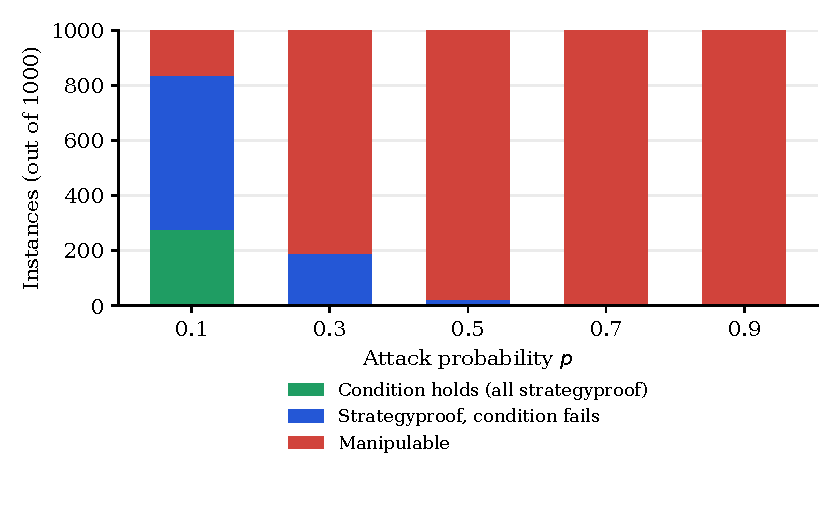
\includegraphics[width=0.68\textwidth]{fig_condition_breakdown.pdf}
\caption{How the sufficient condition relates to measured strategyproofness.}
\label{fig:breakdown}
\end{figure}

\paragraph{The condition never failed to protect.}
There are \emph{zero} instances in which the condition holds but strategyproofness fails; the saved list of such counterexamples is empty. All 285 condition-satisfying instances were strategyproof. This supports the theorem on the sampled population; it does not replace its proof, and a nonzero count would have required checking the witness and the cycle convention before claiming a contradiction.

\paragraph{The condition is far from necessary.}
In 769 instances the mechanism is strategyproof although the condition fails; they are listed in full in \file{results/converse\_examples.json}. In the sample these outnumber the condition-satisfying instances by almost three to one. Their frequency is exactly why a failed condition should not be read as manipulability.

\paragraph{A sparse case: p0.1-trial1.}
Here $A=\{a,\dots,f\}$ with attacks $c\attacks f$, $d\attacks a$, $d\attacks c$, $d\attacks e$, and ownership $\text{Agent 1}=\{a\}$, $\text{Agent 2}=\{d,e,f\}$, $\text{Agent 3}=\{b,c\}$. The condition fails because Agent~2 owns both endpoints of $d\attacks e$. Yet Agent~2 can never do better than utility 2: under full revelation it gets $d$ and $f$ (argument $d$ blocks $c$, which protects $f$), and no report can accept both $d$ and $e$, so it cannot get all three. Hiding $d$ at best swaps $d$ for $e$. Agent~1 owns a single argument and cannot gain by hiding it, and Agent~3 cannot influence $d$ by hiding $b$ or $c$. Strategyproofness is explained without the structural condition.

\paragraph{A dense case: p0.9-trial46.}
With ownership $\text{Agent 1}=\{b,c\}$, $\text{Agent 2}=\{a,d,e\}$, $\text{Agent 3}=\{f\}$, the attacks leave each of the first two agents with at most one acceptable own argument in any conflict-free outcome, and Agent~3 is a singleton. A parity witness still falsifies the condition. The independent audit enumerates 16, 8 and 32 profiles of the other agents respectively and finds a maximum gain from hiding of 0 for every agent. Textbook Example~5.11 gives a more interpretable reason for the same phenomenon: an additional owned defence cancels the indirect self-defeat.

\subsection{Independent audit}
The saved results were re-verified by \file{scripts/audit\_results.py}, which imports none of the production solver code. It computes grounded extensions by integer-bitmask propagation, precomputes every induced outcome, and compares each own report with truthful revelation over all profiles of the others. All 5{,}000 decisions agree, with zero disagreements. This is stronger than reloading a stored strategyproofness flag.

% =====================================================================
\section{Testing}
\begin{table}[H]
\centering
\caption{Automated verification.}
\small
\begin{tabular}{@{}p{3.6cm}p{10.9cm}@{}}
\toprule
Suite & What it checks \\
\midrule
Python unit tests (33) & Definitions and exact textbook expectations, cycles, self-attacks, empty frameworks and agents, tied best responses, invalid ownership and reports. \\
Independent oracles & For all $2^{9}=512$ directed three-node graphs (self-attacks included), enumeration of every total in/out/undec labelling is compared with the production complete, preferred, stable, semi-stable and grounded results; a separate propagation oracle checks strategyproofness on the same space. \\
HTTP and job tests & Routes, input validation, cross-origin rejection, background job lifecycle, failures and recovery, bounded retention, isolation between server instances. \\
Browser tests (24) & Twelve scenarios on desktop and phone viewports with Playwright: graph editing, keyboard toggling of nodes, textbook sets, acceptance changes, hiding incentives, Example~5.11, error messages, import/export, experiments and downloads, responsive layout. \\
Result audit & Independent re-verification of all 5{,}000 saved experiment decisions. \\
\bottomrule
\end{tabular}
\end{table}

All 33 Python tests and all 24 browser tests pass. A GitHub Actions workflow runs the Python suite and the audit on Linux and Windows, and the browser tests on Linux.

% =====================================================================
\section{Limitations and future work}
\begin{itemize}
  \item The algorithms are exact and exponential. The interface caps frameworks at 12 arguments and experiments use 6--8; no claim of scalability is made. SAT or ASP back-ends would be the natural extension for larger graphs.
  \item The experiment uses one seed and a finite sample. More seeds and further probability values would allow tighter statements about the decline in Figure~\ref{fig:sp-fraction}.
  \item The probability values $p$ are provisional, as the assignment text omitted them.
  \item The directed-walk convention for the odd-path condition is conservative; if a simple-path reading is required, the comparison should be repeated (the option exists in the code).
  \item Only abstract frameworks are covered; the structured-argument and dialogue-game mechanisms elsewhere in the chapter are out of scope.
  \item The server is for local demonstration and is not suitable for exposure to the internet.
\end{itemize}

\section{Conclusion}
Argument Lab computes all the required semantics exactly, reproduces the textbook examples (including two errata), and makes the strategic questions explorable. The experiment shows that strategyproofness is common in sparse attack graphs and nearly disappears in dense ones, that the sufficient structural condition of Theorem~5.4 never failed to guarantee truthfulness in 5{,}000 trials, and that it is nevertheless far from necessary: most strategyproof instances violate it. Independent oracles and an independent audit support the correctness of both the engine and the saved results.

% =====================================================================
\section*{Reproducing the results}
\begin{lstlisting}
python server.py                                          # start the application
python -m unittest discover -s tests -v                   # Python tests
python -m argumentation.experiments --count 1000 --seed 2026
python scripts/audit_results.py                           # independent audit
python scripts/make_report_figures.py                     # regenerate the plots
\end{lstlisting}

\begin{thebibliography}{9}
\bibitem{weiss} G.~Weiss (ed.). \emph{Multiagent Systems}, 2nd edition. MIT Press, 2013. Chapter~5, printed pp.~181--185 and 199--201.
\bibitem{rahwan} I.~Rahwan and K.~Larson. Mechanism Design for Abstract Argumentation. In \emph{Proc.\ AAMAS}, 2008.
\bibitem{dung} P.~M.~Dung. On the acceptability of arguments and its fundamental role in nonmonotonic reasoning, logic programming and $n$-person games. \emph{Artificial Intelligence}, 77(2):321--357, 1995.
\end{thebibliography}

\end{document}
